% !TeX root = ../sustechthesis-example.tex

\chapter[离子阱频率稳定]{离子阱频率稳定\label{section:trap_frequency_stablization}}

% \textcolor{red}{这部分主要介绍参考文献\cite[]{Johnson_Wong_Campos_Restelli_Landsman_Neyenhuis_Mizrahi_Monroe_2016}}

带电粒子通常由射频(RF)电势控制,其场梯度提供时间平均力,这些力构成了四极质量滤波器、离子质谱仪和射频(Paul)离子阱等应用的基础\cite[]{Dehmelt_1990, Paul_1990}。这些射频电势,通常在 1 kHz 到 100 MHz 的频率处数百或数千个伏特,在真空中驱动高阻抗负载,通常由射频放大器和谐振升压变换器(例如四分之一波或螺旋谐振器)产生\cite[]{Siverns_Simkins_Weidt_Hensinger_2012}。这种电路容易受到放大器增益、变压器的机械振动和系统中的温度漂移的波动的影响。离子阱对这些波动特别敏感,因为射频电势决定了被捕获离子的谐波振荡频率。稳定的阱频率在从量子信息处理\cite[]{Blatt_Wineland_2008, Monroe_Kim_2013}和量子模拟\cite[]{Richerme_Gong_Lee_Senko_Smith_Foss_Feig_Michalakis_Gorshkov_Monroe_2014, Jurcevic_Lanyon_Hauke_Hempel_Zoller_Blatt_Roos_2014}到原子运动的量子态的制备\cite[]{Leibfried_Blatt_Monroe_Wineland_2003}、原子干涉测量\cite[]{Johnson_Neyenhuis_Mizrahi_Wong_Campos_Monroe_2015}、和量子有限计量\cite[]{Chou_Hume_Koelemeij_Wineland_Rosenband_2010}等方面至关重要。


理论上离子阱中影响阱频率的各种因素
在离子阱系统中,阱频率的表达式为:
\begin{align}
    \omega=e\mu V_0/\sqrt{2}m\Omega R^2
\end{align}

这些参数分别是:
\begin{itemize}
    \item $e$: 离子电荷量;
    \item $\mu$: 几何效率因子;
    \item $m$: 粒子质量;
    \item $R$: 电极间距;
    \item $\Omega$: 输入微波信号的频率;
    \item $V_0$: 输入信号的电压;
\end{itemize}


上面的各个参数中$e$,$\mu$,$m$是常数,R在阱几何形状确定的情况下也是常数。因此,关键的参数在于与射频相关的 $\Omega$ 和 $V_0$ 。这其中,当今射频生成器件自身的频率和幅度稳定性是相当高的,可能产生抖动因素的实际上主要是经过谐振腔后的输出幅度。我们使用的螺线管谐振腔$Q$值较高,只要谐振腔的中心透过频率稍微发生偏移,输出幅度就可能发生较大的抖动。因此阱频稳定主要是通过稳定谐振腔输出的射频幅度实现的。

% 物理上离子阱中影响阱频率的各种因素



\section[离子阱频率稳定原理]{离子阱频率稳定原理}
受环境振动和温度变化影响,谐振腔的几何形状,主要是螺旋线的长度和腔体长度会发生变化,进而导致谐振腔的中心频率发生偏移。从谐振腔的S参数图\ref{fig:helical_compares}中可以看出螺线管谐振腔的Q值很大,透过峰较尖锐,即中心频率附近信号透过衰减较大。因此在输入信号频率抖动极小的情况下,受谐振腔中心频率偏移影响,信号的透过幅度将会发生较大的变化。
文献\cite[]{Johnson_Wong_Campos_Restelli_Landsman_Neyenhuis_Mizrahi_Monroe_2016}中介绍了采用模拟系统实现的离子阱频率稳定方案。该方案的简化版采用了鉴频器、射频功率放大器、模拟PID控制器、电容分压器、混频器、本地振荡源等器件。采用模拟方案涉及到的器件较多、灵活性差,因此我们采用基于数字系统的稳定方式。

基于RTMQ系统的数字PID离子阱频率稳定原理图如图\ref{fig:trap_frequency_lock}所示。信号通过PID对DDS进行幅度调制产生,随后经过射频功率放大器进入谐振腔耦合输入端。通过调节谐振腔耦合输入端对谐振腔进行阻抗匹配耦合,使得输出功率最大化。随后,在输出端焊接一个射频分压电路,按照100:1的分压比采集射频电压作为检测信号送入鉴频器。接着鉴频器的输出接入RTMQ板卡的16位AD转换芯片,进而转换成数字信号作为PID输入,完成整个控制回路闭环。其中,分压电路图如图\ref{fig:trap_frequency_lock}中小图所示,$C_1=C_2\approx10$uF用于同步两个输出端的射频相位;$C_3\approx0.5$pF,$C_4\approx50$pF构成理论上为$100:1$射频分压电路(实际上受到焊接电容影响测得的分压比约为$53:1$)。

\begin{figure}
    \centering
    \caption[数字PID离子阱频率稳定原理图]{基于RTMQ系统的数字PID离子阱频率稳定原理图。DDS:数字频率发生器;PID:比例微分积分控制器;ADC:模拟数字转换器;$C_1,C_2$:相位同步电容;$C_3,C_4$:射频分压电容。\label{fig:trap_frequency_lock}}
    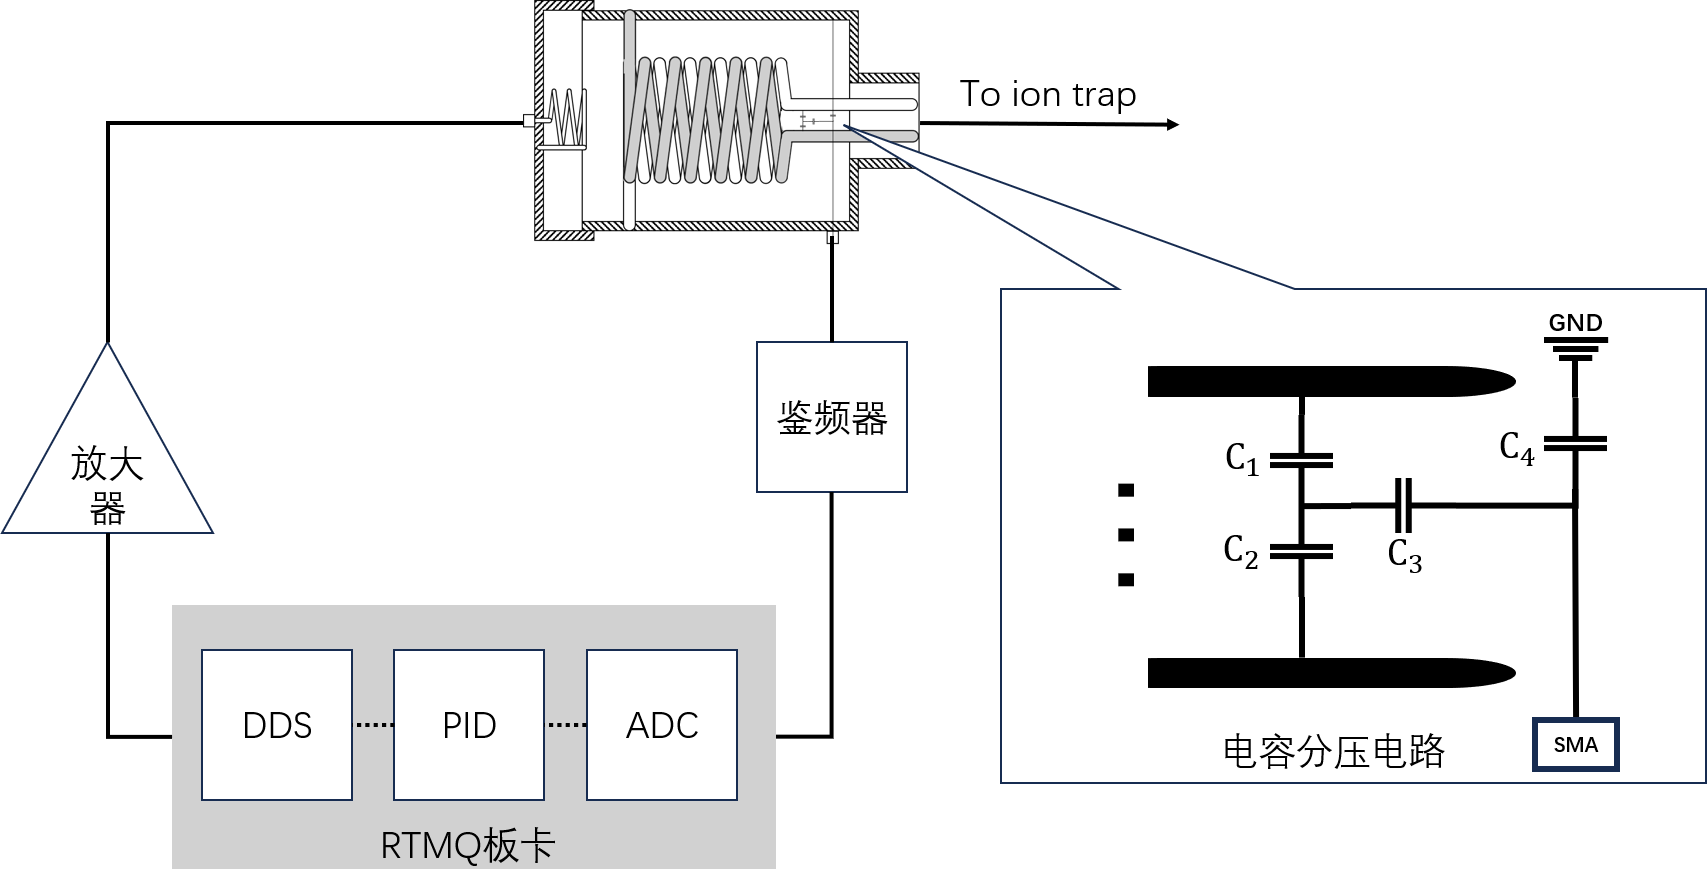
\includegraphics[width=1.0\linewidth]{trap_frequency_lock}
\end{figure}


\section[离子阱频率稳定系统搭建]{离子阱频率稳定系统搭建}

由于系统中需要使用放大器,而放大器对不同频率的信号放大效果有所区别。过大的放大信号可能会损坏谐振腔的分压板,因此这里先用DDS的输出和放大器预先对放大器进行标定,结果如图\ref{fig:helical_lock_amplifier}所示。从结果图中的拟合直线截距上可以看出,信号功率放大器可以对信号放大约32.83dBm。

\begin{figure}
    \centering
    \caption[DDS输出功率和放大器输出功率]{DDS输出功率和放大器输出功率。横坐标为DDS输出功率(单位dBm),纵坐标为测量得到的放大后的射频功率(单位dBm)。蓝色实心点是测得的数据点,蓝色虚线是从数据点中拟合出的直线,系数$a=0.9644$,截距$b=32.83$表示功率放大器的放大dBm数。\label{fig:helical_lock_amplifier}}
    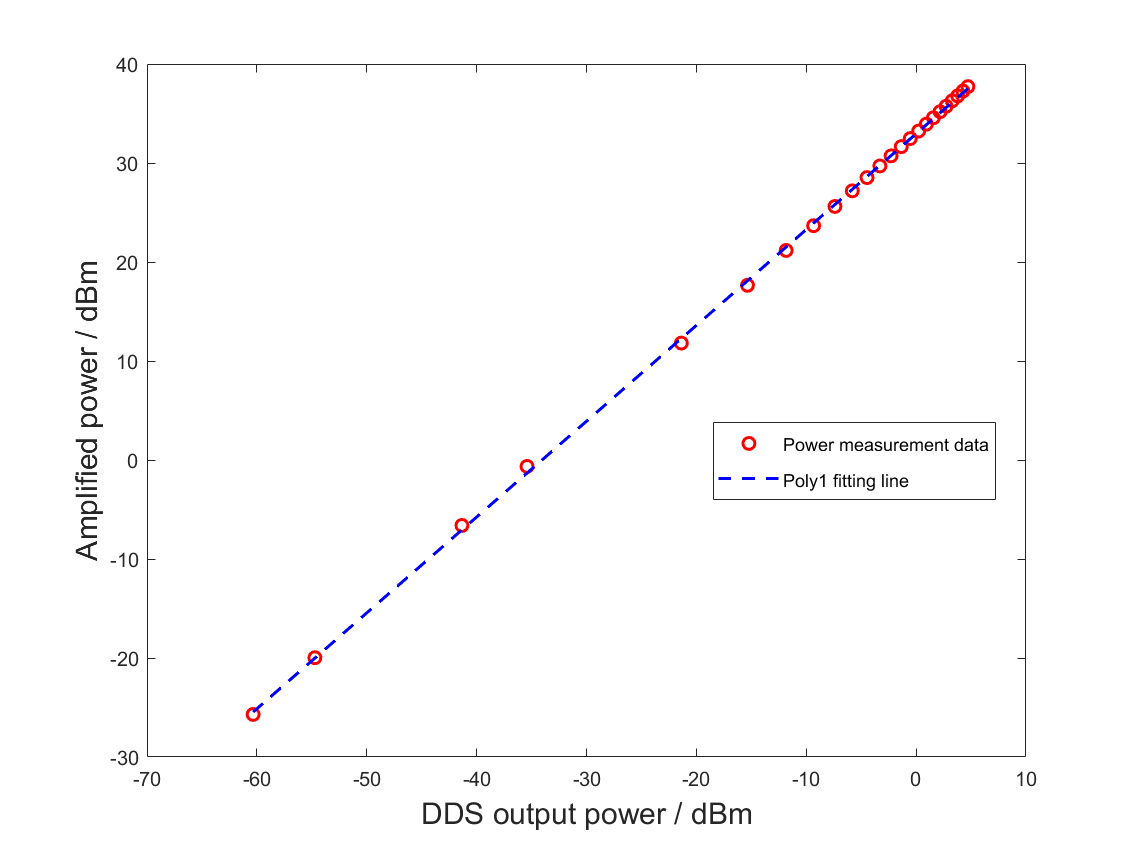
\includegraphics[width=1.0\linewidth]{helical_lock_amplifier}
\end{figure}

阱频稳定模块实验测试图如附录图\ref{fig:trap_frequency_lock_real}所示。

\section[离子阱频率稳定系统结果]{离子阱频率稳定系统结果}

谐振腔输出稳定效果测量结果如图\ref{fig:helical_lock_measure}所示,蓝色测量数据是在未进行稳定时测的的谐振腔输出幅度与输入功率设定值的关系,橙色和灰色测量数据分别为将数字PID控制器目标值设定为-638和-909时的测量结果。在未稳定的情况下,谐振腔的输出幅度会跟随外部输入信号的幅度变化而变化,呈现出一定的比率关系。如图中蓝色测量数据,其斜率约为244.55;经过稳定后,在大范围内谐振腔的输出幅度仍然会跟随外部输入信号的幅度变化而变化,不过其呈现的比例关系会受到稳定抑制作用而减小,如图中橙色和灰色测量数据,其斜率在155附近。从中可见,添加数字PID控制器对谐振腔的输出幅度会有明显的稳定抑制作用。

\begin{figure}
    \centering
    \caption[谐振腔输出稳定效果测量结果]{谐振腔输出稳定效果测量结果。横坐标为DDS的设定输出功率数字值(非实际功率值),纵坐标我板卡上ADC测得的输出电压数字值(非实际功率值)。该图个数据点测量的是PID参考功率数值一定的情况下,改变输入的射频功率大小,看实际输出功率大小的变化。整体上斜率越小表明控制器对功率大小的变化有抑制作用。\label{fig:helical_lock_measure}}
    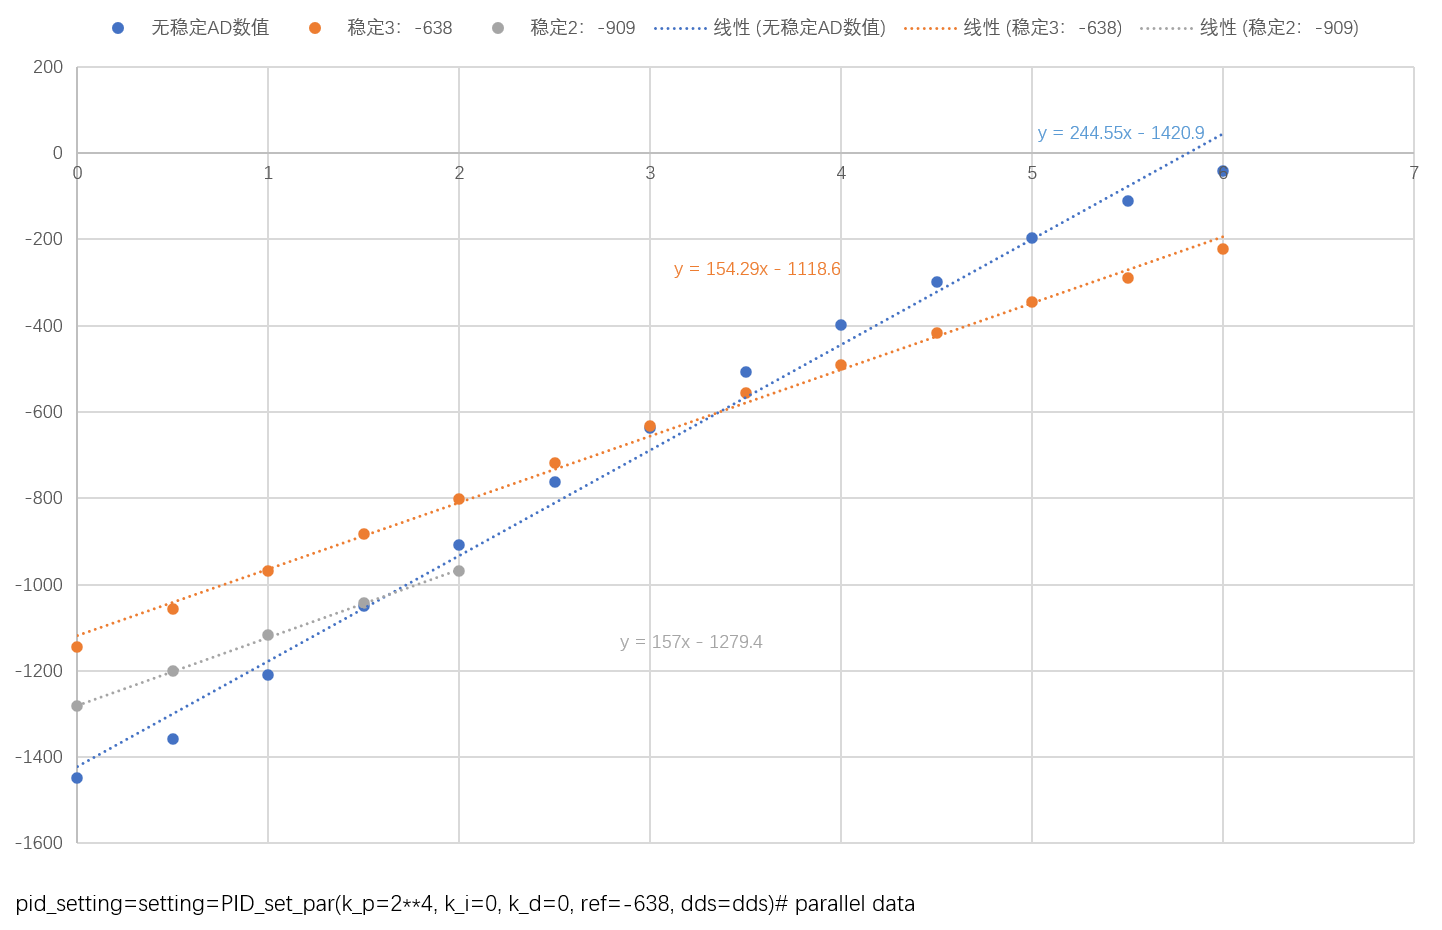
\includegraphics[width=1.0\linewidth]{helical_lock_measure}
\end{figure}


